\documentclass[11pt]{amsart}
\usepackage{geometry}                % See geometry.pdf to learn the layout options. There are lots.
\geometry{letterpaper}                   % ... or a4paper or a5paper or ... 
%\geometry{landscape}                % Activate for for rotated page geometry
%\usepackage[parfill]{parskip}    % Activate to begin paragraphs with an empty line rather than an indent
\usepackage{graphicx}
\usepackage{color}
\usepackage{listings}
\usepackage{amssymb}
\usepackage{epstopdf}
%\usepackage{tikz}
\usepackage{bm}
\usepackage{tkz-euclide}
\usetkzobj{all}
\newcommand{\Sinc}{\operatorname{Sinc}}

\DeclareGraphicsRule{.tif}{png}{.png}{`convert #1 `dirname #1`/`basename #1 .tif`.png}

\lstset{language=Matlab, 
	mathescape=true,
    	basicstyle = \sffamily
} 


\title{Notes for the Boltzmann equation and its Fast Spectral Methods}
\author{Lianhua Zhu}
%\date{}                                           % Activate to display a given date or no date

\begin{document}
\maketitle
\section{The Boltzmann collision term}
\subsection{Binary collision dynamics}

%\subsection{}


Firstly, the relative speed before collision is
\begin{equation}
g \triangleq v-v_*, \quad r \triangleq |g|.
\end{equation}

The post-collision speed can be derived by the constraints that the relative speed and mean velocity  are not changed before and after the collision:
\begin{equation}
\frac{1}{2} (v')^2 + \frac{1}{2}(v'_*)^2 = \frac{1}{2} (v)^2 + \frac{1}{2}(v_*)^2
\end{equation}

\begin{equation}\label{eq:vprimsum}
v' + v'_* = v + v_*
\end{equation}

Assuming $\omega$ is the unit vector on the sphere whose center locate at $v-v_*$ and $\omega$ points to the direction of $v'-v_*'$, i.e.,
\begin{equation}\label{eq:vprimdiff}
v' - v'_* =  |v-v_*| \omega = r\omega.
\end{equation}

From Eq.~\eqref{eq:vprimsum} and \eqref{eq:vprimdiff} we obtains:
%So we have 8 unknown scalar (3 in $v'$, 3 in $v'_*$ and 2 in $\omega$) and eight scalar equations. 
\begin{equation}
v' = v - {g\over2} + {r\over2} \omega,\quad v'_* = v - {g\over2} - {r\over2} \omega
\end{equation}


% If instead we know only $v$ and $|v-v'|$ and $\omega$ then we can solve the full $v_*$ and $v'$ and $v'_*$
\subsection{The collision integral in different forms}
 The collision terms is an 5-fold integral (three in $dv_*$, one in impact parameter $b$ and one in impact plane angle $d\epsilon$):
\begin{equation}
\Omega(f)(v) 
=  \int_{\mathbb{R}^3} \int_0^{+\infty} \int_0^{2\pi} [f(v_*')f(v')-f(v_*)f(v')] r bdbd\epsilon dv_* 
\end{equation}
Change to use deflection angle $\chi$ instead of impacting parameter ($b$):
\begin{equation}
bdbd\epsilon =  \sigma d\omega  = \frac{b}{\sin\chi}\left|\frac{db}{d\chi}\right|d\chi d\epsilon 
		   = \frac{b}{\sin \chi} \left|\frac{db}{d\chi}\right|d\omega 
		   \triangleq  \frac{1}{r} {B}(r,\cos\chi) d\omega
\end{equation}
Note, the deflection angle is the angle between the pre- and post-collision relative velocity, i.e.,
\begin{equation}
\cos \chi = {\omega \cdot g \over r}
\end{equation}

Then we have the following equivalent forms of the collision term:
\begin{align}
\begin{split}
Q(f,f)(v) 
&=  \int_{\mathbb{R}^3} \int_0^{+\infty} \int_0^{2\pi} [f(v_*')f(v')-f(v_*)f(v)] r bdbd\epsilon dv_* \\
&=  \int_{\mathbb{R}^3} \int_0^{\pi} \int_0^{2\pi} [f(v_*')f(v')-f(v_*)f(v)] r \frac{b}{\sin \chi} \left|\frac{db}{d\chi} \right| d\chi d\epsilon dv_* \\
&=  \int_{\mathbb{R}^3} \int_0^{\pi} \int_0^{2\pi} {B}(r,\cos\chi)[f(v_*')f(v')-f(v_*)f(v)] d\chi d\epsilon dv_* \\
&=  \int_{\mathbb{R}^3} \int_{\mathcal{S}^2} {B}(r,\cos\chi)[f(v_*')f(v')-f(v_*)f(v)] d\omega dv_* \\
&=  \int_{\mathbb{R}^3} \int_{\mathcal{S}^2} r \sigma(r,\cos\chi)[f(v_*')f(v')-f(v_*)f(v)] d\omega dv_* \\
&=  \int_{\mathbb{R}^3} \int_{\mathcal{S}^2} {B}(r,\cos\chi)[f(v_*')f(v')-f(v-g)f(v)]d\omega dg \\
& = Q^{+}(f,f) - Q^{-}(f,f) \\
& = Q^{+}(f,f) - fL(f)
\end{split}
\end{align}
in which here $\sigma(r,\cos\chi) = (b/\sin \chi) |\text{d} b/\text{d} \chi|$ is called the differential cross-section (DCS). $L(f)$ is
\begin{equation}
L(f) \triangleq \int_{\mathbb{R}^3} \int_{\mathcal{S}^2} {B}(r,\cos\chi)f(v-g)d\omega dg
\end{equation}

The \emph{total collision cross-section} (TCS) $\sigma_T$ is defined as
\begin{equation}
\sigma_T = \int_0^{4\pi} \sigma d\omega
\end{equation}

For hard sphere:
\begin{equation}
\sin\left[\frac{1}{2}(\pi - \chi)\right]=\frac{b}{d_{HS}} \to  \chi = 2\cos^{-1}\frac{b}{d_{HS}}
\end{equation}
Therefore
\begin{equation}
\left| {db\over d\chi} \right| = {1\over 2}d_{HS}\sin(\chi/2)
\end{equation}
and note that $b = d_{HS} \cos(\chi/2)$, we have
\begin{equation}
\sigma = \frac{d_{HS}^2}{4}
\end{equation}

\begin{figure}[htbp]
\begin{center}
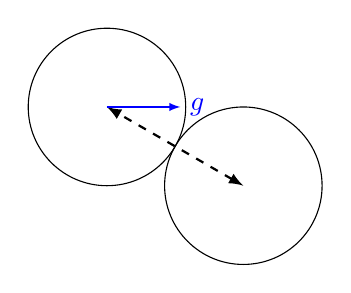
\begin{tikzpicture}
 % \tkzInit[xmax=4,ymax=4,xmin=-4,ymin=-4]
 %  \tkzGrid
 %  \tkzAxeXY
  % \draw[ thick,-latex] (-6,0) -- (6,0) node [anchor= west]{$x$};
   %\draw[ thick,-latex] (0,-6) -- (0,6) node [anchor= west]{$x$};
   \draw[] (0,0) circle (1);
   \draw[] (-1.732,1) circle (1);
   \draw[ thick,dashed,latex-latex] (0,0) -- (-1.732,1);
   \draw[blue, -latex] (-1.732,1) -- (-0.8, 1) node [right] {$g$};

 % \tkzText[above](0,6.75){2D demo of the basic identity}
  \end{tikzpicture}
\caption{For any point $x$ on the blue circle, the projection point of $u$ on $-x$ should be $-x/2$.}
\label{fig:identity}
\end{center}
\end{figure}


For VHS model, the $B$ is only a function of $r$ and does not depends on $\cos \chi$:
\begin{equation}
 {B}(r,\cos\chi) =  b_\gamma r^\gamma
\end{equation}
in which $\gamma = 0$ corresponds to Maxwell model and $\gamma = 1$ corresponds to HS mode. $b_\gamma = d_{HS}^2/4$ for HS model.


\section{Gauss Legendre quadrature}
\begin{equation}
\int_{a}^{b} f(t) d t=\frac{b-a}{2} \sum_{k=1}^{N} w_{N, k} f\left(\frac{a+b}{2}+\frac{b-a}{2} x_{N, k}\right)
\end{equation}

\section{Fourier transformation and convolution}

\subsection{Complex number}
\begin{equation}
e^{ix} = \cos x + i \sin x
\end{equation}

\subsection{Frequency}
The relation between the frequency $f$ and the angular frequency  $\omega$ is
\begin{equation}
\omega=\frac{2 \pi}{T}=2 \pi f.
\end{equation}
A sine signal with period of $T$  is represented is $\sin(\omega t) = \sin(\frac{2\pi}{T}t) = \sin(2\pi f t) $


\subsection{Integration of sine and cosine functions}

\begin{equation}
\int_0^{2\pi}\cos (mt) \cos (nt)  dt 
\end{equation}

\subsection{Fourier serials}
A periodical function $f(t)$ with period of T, can be approximated using the following \emph{Fourier series}:
\begin{equation}
g(t) = a_0 + \sum_{m=1}^{\infty} a_m\cos \left(\frac{2\pi m t}{T}\right )  + \sum_{m=1}^{\infty} b_m\sin \left(\frac{2\pi m t}{T}\right )
\end{equation}
It means the original $f(t)$ can be approximated using the summation of a serial sine and cosine functions with period of $T$, $T/2$, $T/3$, $\cdots$, etc. 
Note the $f(t)$ is not necessarily to be smooth or continuous. A pulse function can be approximated using such an expansion as well.


The coefficients are determined as

\begin{align}
\begin{split}
a_0 & = {1\over T}\int_0^T f(t)dt \\
a_m &= {2\over T}\int_0^T f(t) \cos \left(\frac{2\pi m t}{T}\right )  dt  \\
b_m &= {2\over T}\int_0^T f(t) \sin \left(\frac{2\pi m t}{T}\right )  dt 
\end{split}
\end{align}

Writing the Fourier serial in complex form
\begin{equation}
g(t) = \sum_{n = -\infty}^{\infty} c_n e^{i\frac{2\pi n}{T}t}.
\end{equation}
Now the coefficient in complex form is
\begin{equation}
c_n = {1\over T}\int_0^T f(t) e^{-i\frac{2\pi n}{T}t}dt.
\end{equation}
Note $c_n$ is complex number. If $c^*_n = -c_{-n}$, then $g(t)$ will be entirely real. 

\subsection{DFS (Discrete Fourier  Series)}
When the $f(t)$ are discretely defined (sampled) on a serial of equaly spaced points $t_m = mT/N,~(m = 0, 2., \ldots, N-1)$ as $f[m]$. Then we have (replace $n$ with $k$)
\begin{equation}
c_k = \frac{1}{N} \sum_{m=0}^{N-1}f[m] e^{-i\frac{2\pi k}{T}t_m} = 
 \frac{1}{N} \sum_{m=0}^{N-1}f[m] e^{-i\frac{2\pi}{N}mk}, k = 0, \ldots N
\end{equation}
The components	other then those in $0, \ldots N$ are not defined. The discrete samples are recovered as
\begin{equation}
f[m] =  \sum_{k=0}^{N-1}c_k e^{i\frac{2\pi k}{N}mk}, k = 0, \ldots N
\end{equation}

%If we considering use a continuous spectral of sine/cosine functions to approximate $f(t)$, then we have the Fourier transformation of 
%\begin{equation}
%F(\omega) \triangleq \mathcal{F}(f(t))= \frac{1}{T}\int_0^{T}f(t)e^{-i\omega t}dt
%\end{equation}

\subsection{DFT (Discrete Fourier Transformation)}
The $N$-point DFT of of signal of $f[m]$ is formally \emph{defined} as
\begin{equation}
F[k] =  \sum_{m=0}^{N-1}f[m]e^{-i\frac{2\pi}{N}mk} = N c_k
\end{equation}
{\color{red}Note that in this definition, there is no $1/N$ before the summation as in the DFS.}
And the Inverse DFT (IDFT) is
\begin{equation}\label{idft}
f[m] = \frac{1}{N} \sum_{k=0}^{N-1}F[k] e^{i\frac{2\pi}{N}mk}, m = 0, \ldots N
\end{equation}
The 3D equivalent are
\begin{equation}
F[k] =  \sum_{m=0}^{N-1}f[m]e^{-i\frac{2\pi}{N}m\cdot k},
\end{equation}
and
\begin{equation}
f[m] = \frac{1}{N^3} \sum_{k=0}^{N-1}F[k] e^{i\frac{2\pi}{N}k\cdot m}.
\end{equation}
where $m$, $n$ and $k$ are 3-component indexes, i.e., each component of them (e.g., $m_1$, $m_2$ and $m_3$) are from $0$ to $N-1$.

\subsection{Convolution}

The \emph{convolution} of functions $f(t)$ and $g(t)$ is 
\begin{equation}
(f*g)(t) \triangleq \int_{-\infty}^{\infty}f(\tau)g(t-\tau)d\tau
\end{equation}
When the convolution on functions $f$ and $g$ defined in bounded domain $[0, T]$ is
\begin{equation}
(f*g)(t) \triangleq \int_{0}^{T}f(\tau)g(t-\tau)d\tau, \
\end{equation}

\subsubsection{Periodic summation}
Any periodic function, $s_{T}(t)$ with period T, can be represented by a summation of an infinite number of instances of an aperiodic function, $s(t)$ that are offset by integer multiples of  $T$, and the representation is called \emph{periodic summation}:
\begin{equation}
s_{P}(t)=\sum_{n=-\infty}^{\infty} s(t+n P)=\sum_{n=-\infty}^{\infty} s(t-n P).
\end{equation}

\subsubsection{Continuous circular convolution}
When a function $g_T$ is periodic, with period $T$, then for function $f$, such that $f*g_T$ exists, the convolution is also periodic and identical to:
\begin{equation}
\left(f*g_{T}\right)(t) \equiv \int_{t_{0}}^{t_{0}+T}\left[\sum_{k=-\infty}^{\infty} f(\tau+k T)\right] g_{T}(t-\tau) d \tau
\end{equation}
where $t_0$ is an arbitrary choice.

\subsubsection{Discrete linear convolution}
If $f$ and $g$ are both defined on the whole integer set $\mathcal{Z}$, the \emph{discrete convolution} of them is given by 
\begin{equation}\label{dlc}
(f*g)[k] = \sum_{m=-\infty}^{\infty}f[m]g[k-m]
\end{equation}
Or
\begin{equation}
(f*g)(k) = \sum_{\substack{m,n = -\infty \\ m+n = k} }^{\infty}f[m]g[n],
\end{equation}
When  $f$ and $g$ are defined only on a finite sequence $1, 2, \ldots, N$ and  the definition Eq.\eqref{dlc} is defined by extending the sequences to finitely supported functions on the set of integers.
\begin{equation}
(f*g)(k) = \sum_{\substack{m, n = 0 \\ m+n = k} }^{N-1}f[m]g[n],\quad k = 1, 2, \ldots, 2N-1
\end{equation}

 When the sequences are the coefficients of two polynomials, then the coefficients of the ordinary product of the two polynomials are the convolution of the original two sequences. This is known as the Cauchy product of the coefficients of the sequences. The discrete convolution of two finite sequences can be calculated in Matlab like 
 \begin{lstlisting}
>> conv([2,0,1],[3,1])
ans =
     6     2     3     1
\end{lstlisting}
The linear convolution of an $M$-point vector, $x$, and an $N$-point vector, $y$, has length $N + M - 1$.

\subsubsection{Discrete circular convolution}
 For two vectors, $x$ and $y$, the \emph{circular convolution} is equal to the inverse discrete Fourier transform (IDFT) of the \emph{element-wise} product of the vectors' DFTs. If $x$ and $y$ have different length, say $M$ and $N$, they have to be padded with \emph{enough zeros} to use the DFT, e.g., following the last Matlab example,
\begin{lstlisting}
M = length(x);
N = length(y);
xpad = [x zeros(1, N-1)];
ypad = [y zeros(1, M-1)];
ccirc = ifft(fft(xpad).*fft(ypad))
ccirc =
    2.0000    5.0000   10.0000    8.0000    8.0000    3.0000
\end{lstlisting} 
The Signal Processing Toolbox software of Matlab has a function, \verb|cconv|,  the linear convolution of x and y using circular convolution with the following code:
\begin{lstlisting}
ccirc2 = cconv(x,y,M+N-1);
\end{lstlisting} 

%If both $f$ and $g$ are sampled uniformly on $N$ points $t_m = mT/N, ~~ m = 0, \ldots, N-1$, then we can define the \emph{discrete circular convolution} as
%\begin{equation}
%(f*g)[k] = \sum_{m =0}^{N-1}f[m]g[k-m], \quad k = 0, 1, \ldots, 2N-1
%\end{equation}

\subsubsection{Circular convolution theorm}
The \emph{circular convolution} is equal to the inverse discrete Fourier transform (IDFT) of the \emph{element-wise} product of the (zero padded) vectors' DFTs, i.e.,
\begin{equation}
(f*g)[k] = \mathcal{F}^{-1}( \mathcal{F}(f_{zp})\cdot \mathcal{F}(g_{zp}))
\end{equation}
or
\begin{equation}
\mathcal{F}((f*g)) = \mathcal{F}(f_{zp})\cdot \mathcal{F}(g_{zp})
\end{equation}
where the symbol `$\cdot$' is element-wise product and the subscript $p$ means zero-padded. Below is a simple proof.

By using Eq.~\eqref{idft},
\begin{equation}
(f*g)[k] = \sum_{\substack{m,n = 0 \\ m+n = k} }^{N-1} \left( \frac{1}{N^3} \sum_{p=0}^{N-1}F[p] e^{i\frac{2\pi}{N}m\cdot p} \right)  \left( \frac{1}{N^3} \sum_{q=0}^{N-1}G[q] e^{i\frac{2\pi}{N}n\cdot q} \right)
\end{equation}
Supposing $F[p]$, $G[q]$ are the DFTs of  $f$ and $g$, respectively
\begin{align}
\begin{split}
\mathcal{F}((f*g)[k])[l] &=   \sum_{k=0}^{2N-1}\left[  \sum_{\substack{m,n = 0 \\ m+n = k} }^{N-1} \left( \frac{1}{N^3} \sum_{p=0}^{N-1}F[p] e^{i\frac{2\pi}{N}m\cdot p} \right)  \left( \frac{1}{N^3} \sum_{q=0}^{N-1}G[q] e^{i\frac{2\pi}{N}n\cdot q} \right) \right] e^{-i \frac{2\pi}{N}k\cdot l}\\\end{split}
\end{align}
where $l = 1, 2, \ldots, 2N-1$. N.B. The proof is left to future investigation.


%% Some difference in the definition of DFT
%When the $f(t)$ are discretely defined (sampled) on a serial of equality spaced $t_m = m\frac{T_0}{N},~(m = 0, 2., \ldots, N-1)$, then we can regard each sample $f[k]$ as impulse functions. Then we have 
%\begin{equation}
%F(\omega) =   \frac{1}{N} \sum_{m=0}^{N-1}f[m]e^{-i\omega t_m}
%\end{equation}
%We interested only in the fundamental frequencies $\omega_k$ as
%\begin{equation}
%\omega = 0, \frac{2\pi}{T}, 2\frac{2\pi}{T}, 3\frac{2\pi}{T}, \ldots , (N-1)\frac{2\pi}{T}
%\end{equation}
%The amplitude for each component is is the discrete Fourier transformation 
%\begin{equation}
%F[k] = F(\omega_k) =   \frac{1}{N} \sum_{m=0}^{N-1}f[m]e^{-i \frac{2\pi}{T}k  t_m} =  \frac{1}{N} \sum_{m=0}^{N-1}f[m]e^{-i \frac{2\pi}{N}km} 
%\end{equation}

\subsection{An example}
Considering $f = [9, 4, 8, 0]$, then $$
F[k]=\sum_{0}^{3} f[m] e^{-i \frac{\pi}{2} m k}=\sum_{k=0}^{3} f[k](-i)^{mk}
$$

$$
\left( \begin{array}{c}{F[0]} \\ {F[1]} \\ {F[2]} \\ {F[3]}\end{array}\right)=\left( \begin{array}{cccc}{1} & {1} & {1} & {1} \\ {1} & {-i} & {-1} & {i} \\ {1} & {-1} & {1} & {-1} \\ {1} & {i} & {-1} & {-i}\end{array}\right) \left( \begin{array}{c}{f[0]} \\ {f[1]} \\ {f[2]} \\ {f[3]}\end{array}\right)=\left( \begin{array}{c}{20} \\ {-i 4} \\ {12} \\ {i 4}\end{array}\right)
$$
Verify with Matlab:

 \begin{lstlisting}
>> fft([8,4,8,0]')
ans =
  20.0000 + 0.0000i
   0.0000 - 4.0000i
  12.0000 + 0.0000i
   0.0000 + 4.0000i   
 >> ifft(ans)'
ans =
    8     4     8     0
 \end{lstlisting}

\subsection{FFT (fast Fourier transformation)}

Discrete Fourier transformation by the fast Fourier transformation (FFT) efficiently. 

Below is an Matlab example for the FFT of a discrete equilibrium distribution function
 \begin{lstlisting}
N = 32;
x = linspace(-6,6,N);
f = exp(-x.*x/2)/sqrt(2*pi);
y = fft(fftshift(f));
ff = fftshift(ifft(y));
plot(x,f);
hold on;
plot(x,ff,'ro');
\end{lstlisting}
 


\subsection{Convolution using FFT}

\subsubsection{Definition of convolution}
Definition of the convolution of two functions $f$ and $g$:
\begin{equation*}
(f*g)(x) \triangleq \int_ {-\infty}^{\infty}f(\tau)(t-\tau)d\tau
\end{equation*}


In Matlab, \verb|w = conv(u,v)| returns the \emph{circular convolution} of vectors \verb|u| and \verb|v|. If  \verb|u| and \verb|v| are vectors of polynomial coefficients, convolving them is equivalent to multiplying the two polynomials. For example, we have $p_1 = 2x^2 + 6$, and $p_2 = x^3 + 3x$, then we have $ u = [2, 0, 6]$ and $v = [1, 0,3,0]$ as the coefficients of $p_1$ and $p_2$ respectively. The multiplication of $p_1$ and $p_2$ are 
\begin{equation}
p = p_1 p_2 = (2x^2 + 6) (x^3 + 3x) = 2x^5 + 0 x^4 + 12 x^3 + 0x^2 + 18 x + 6.
\end{equation}
So $w = conv(u,v) =  [2,0,9,0,18,6]$.

\subsection{Convolution theorem} Under suitable conditions the Fourier transform of a convolution of two signals is the point-wise product of their Fourier transforms. In other words, convolution in one domain (e.g., time domain) equals point-wise multiplication in the other domain (e.g., frequency domain). 

\begin{equation}
\mathcal{F}\{f*g\}  =  k \cdot \mathcal{F}\{f\} \cdot  \mathcal{F}\{g\}
\end{equation}


Keep in mind that the product of the DFTs of two vectors is Fourier transform of the \emph{circular convolution}, not linear convolution. To establish equivalence between linear and circular convolution, you have to extend the vectors appropriately first before computing the circular convolution. The length of the linear convolution of two vectors of length, M and L is M+L-1, so we will extend our two vectors to that length before computing the circular convolution using the DFT.
 
 \begin{lstlisting}
 x = [5 6 8 2 5]; 
 y = [6 -1 3 5 1];
 x1 = [x zeros(1,4)];
 y1 = [y zeros(1,4)];
 c1 = ifft(fft(x1).*fft(y1));
 c2 = conv(x,y);
 \end{lstlisting}

 \section{FSM on the collision integral}
The spectral method of the BE collision term has been explained in detail in 
 \cite{pareschiNumericalSolutionBoltzmann2000}.
 
 \subsection{DFT on 3D distribution function}
Discretize the velocity space in a bound domain of $[-L,L]^3$ with uniform velocity grid points  $v_m = m \frac{2L}{N}, m =  -N/2, \ldots, N/2-1$, we have the discrete distribution function as $f_m \triangleq f(v_m)$. 
\begin{equation}
 f_N(v) = \sum_{k = -N/2}^{N/2-1}\hat f_k e^{i{\pi \over L}k\cdot v}
\end{equation}

\begin{equation}
\hat f_k = \frac{1}{(2L)^3}\int_\mathcal{D_L} f(v) e^{-i {\pi \over L} k \cdot v}dv 
%= \frac{1}{N^3} \sum_{m=-N/2}^{N/2-1}f(v_m)e^{-i \frac{\pi}{L}k\cdot v_m}
\end{equation}

\color{blue}
Note in Matlab DFT and IDFT, the accusation definition is a little different
\begin{equation}
 f[m] = \frac{1}{N^3}\sum_{k = -N/2}^{N/2-1}\hat f[k] e^{i{\pi \over L}k\cdot v_m}
\end{equation}
\begin{lstlisting}
f = fftshift(fftn(fftshift(fF)));
\end{lstlisting}
\begin{equation}
\hat f[k] = \sum_{m = -N/2}^{N/2-1}  f[m] e^{-i {\pi \over L} k \cdot v_m} 
%= \frac{1}{N^3} \sum_{m=-N/2}^{N/2-1}f(v_m)e^{-i \frac{\pi}{L}k\cdot v_m}
\end{equation}
\begin{lstlisting}
fF = fftshift(ifftn(fftshift(f)));
\end{lstlisting}

\color{black}
\begin{align*}
\begin{split}
fL(f) &= f(v)\int_{\mathbb{R}^3} \int_{\mathcal{S}^2} {B}(r,\cos\chi)f(v-g)d\omega dg \\
\end{split}
\end{align*}

\begin{align*}
\begin{split}
f_NL(f_N) &=  \sum_{l = -N/2}^{N/2-1}\hat f_l e^{i{\pi \over L}l\cdot v} \int_{\mathbb{R}^3} \int_{\mathcal{S}^2} {B}(r,\cos\chi)   \sum_{m = -N/2}^{N/2-1}\hat f_m e^{i{\pi \over L}m\cdot (v-g)} d\omega dg \\
&=  \sum_{l = -N/2}^{N/2-1}\sum_{m = -N/2}^{N/2-1}\hat f_l \hat f_m  \int_{\mathcal{S}^2} {B}(r,\cos\chi)  e^{-i{\pi \over L}mg} d\omega dg e^{i{\pi \over L}(l+m)\cdot v}
\end{split}
\end{align*}

\color{blue}
\begin{align*}
\begin{split}
f_NL(f_N) &= \frac{1}{N^3} \sum_{l = -N/2}^{N/2-1}\hat f[m] e^{i{\pi \over L}l\cdot v} \int_{\mathbb{R}^3} \int_{\mathcal{S}^2} {B}(r,\cos\chi)  \frac{1}{N^3} \sum_{m = -N/2}^{N/2-1}\hat f[m] e^{i{\pi \over L}m\cdot (v-g)} d\omega dg \\
&=  \frac{1}{N^6}\sum_{l = -N/2}^{N/2-1}\sum_{m = -N/2}^{N/2-1}\hat f[l]\hat f[m] \int_{\mathbb{R}^3} \int_{\mathcal{S}^2} {B}(r,\cos\chi)  e^{-i{\pi \over L}mg} d\omega dg e^{i{\pi \over L}(l+m)\cdot v}
\end{split}
\end{align*}
\color{black}


\begin{align*}
\begin{split}
Q^{+}(f,f)&=  \int_{\mathbb{R}^3} \int_{\mathcal{S}^2} {B}(r,\cos\chi) f(v_*')f(v')d\omega dg \\
\end{split}
\end{align*}

\begin{equation}
v' = v - {g\over2} + {r\over2} \omega,\quad v'_* = v - {g\over2} - {r\over2} \omega
\end{equation}

\begin{align*}
\begin{split}
Q^{+}(f_N,f_N)&=  \int_{\mathbb{R}^3} \int_{\mathcal{S}^2} {B}(r,\cos\chi) f_N(v - {g\over2} - {r\over2}\omega)f_N( v - {g\over2} + {r\over2}\omega)d\omega dg \\
&=  \int_{\mathbb{R}^3} \int_{\mathcal{S}^2} {B}(r,\cos\chi)  \sum_{l = -N/2}^{N/2-1}\hat f_l e^{i{\pi \over L}l\cdot (v - {g\over2} - {r\over2}\omega)}  \sum_{m = -N/2}^{N/2-1}\hat f_m e^{i{\pi \over L}m\cdot (v - {g\over2} + {r\over2}\omega)}d\omega dg \\
&= \sum_{l = -N/2}^{N/2-1} \sum_{m = -N/2}^{N/2-1} \hat f_l \hat f_m  \int_{\mathbb{R}^3} \int_{\mathcal{S}^2} {B}(r,\cos\chi) e^{i{\pi \over L}l\cdot (- {g\over2} + {r\over2}\omega)} e^{i{\pi \over L}m\cdot (- {g\over2} - {r\over2}\omega)}d\omega dg e^{i{\pi \over L}(l+m)\cdot v}\\
&= \sum_{l = -N/2}^{N/2-1} \sum_{m = -N/2}^{N/2-1} \hat f_l \hat f_m  \int_{\mathbb{R}^3} \int_{\mathcal{S}^2} {B}(r,\cos\chi) 
e^{-i{\pi \over L} g \frac{l+m}{2} -i {\pi \over L} r\omega \frac{m-l}{2}}
d\omega dg e^{i{\pi \over L}(l+m)\cdot v}\\
\end{split}
\end{align*}

\color{blue}
\begin{align*}
\begin{split}
Q^{+}(f_N,f_N)&= \frac{1}{N^6}\sum_{l = -N/2}^{N/2-1} \sum_{m = -N/2}^{N/2-1} \hat f[l] \hat f[m]  \int_{\mathbb{R}^3} \int_{\mathcal{S}^2} {B}(r,\cos\chi) 
e^{-i{\pi \over L} g \frac{l+m}{2} -i {\pi \over L} r\omega \frac{m-l}{2}}
d\omega dg e^{i{\pi \over L}(l+m)\cdot v}\\
\end{split}
\end{align*}
\color{black}

To unify the representation of $f_NL(f_N)$ and $Q^{+}(f_N)$, define the following expression
\begin{equation*}
G(l,m) \triangleq \int_{\mathbb{R}^3} \int_{\mathcal{S}^2} {B}(r,\cos\chi) 
e^{-i{\pi \over L}\frac{l+m}{2} \cdot g -i {\pi \over L} r \frac{m-l}{2}\cdot \omega}d\omega dg 
\end{equation*}
Then we have
\begin{equation*}
f_NL(f_N) = \sum_{l = -N/2}^{N/2-1}\sum_{m = -N/2}^{N/2-1}\hat f_l \hat f_m G(m,m) e^{i{\pi \over L}(l+m)\cdot v}
\end{equation*}
\begin{equation*}
Q^{+}(f_N,f_N) =  \sum_{l = -N/2}^{N/2-1}\sum_{m = -N/2}^{N/2-1}\hat f_l \hat f_m G(l,m) e^{i{\pi \over L}(l+m)\cdot v}
\end{equation*}

\color{blue}
\begin{equation*}
f_NL(f_N)(v) = \frac{1}{N^6} \sum_{l = -N/2}^{N/2-1}\sum_{m = -N/2}^{N/2-1}\hat f[l] \hat f[m] G(m,m) e^{i{\pi \over L}(l+m)\cdot v}
\end{equation*}
\begin{equation*}
Q^{+}(f_N,f_N)(v) =  \frac{1}{N^6} \sum_{l = -N/2}^{N/2-1}\sum_{m = -N/2}^{N/2-1}\hat f[l] \hat f[m] G(l,m) e^{i{\pi \over L}(l+m)\cdot v}
\end{equation*}
\color{black}

\begin{align*}\begin{split}
\hat Q_k &=    \frac{1}{(2L)^3}\int_\mathcal{D_L} Q(f_N)e^{-i{\pi \over L}k\cdot v} dv =  \textcolor{red}{\frac{1}{N^3}}\sum_{\substack{l,m= -N/2 \\ l+m = k}}^{N/2-1}\mathcal{G}(l,m)\hat f_l  \hat f_m
\end{split}\end{align*}

\begin{align*}\begin{split}
\mathcal{G}(l,m) = G(l,m) - G(m,m)
\end{split}\end{align*}

\color{blue}
\begin{align*}\begin{split}
\hat Q[k] &=  \sum_{q=-N/2}^{N/2-1} Q[q]e^{-i{\pi \over L}k\cdot v_q}=   \frac{1}{N^3} \sum_{\substack{l,m= -N/2 \\ l+m = k}}^{N/2-1}\mathcal{G}(l,m)\hat f[l] \hat f[m]  \\
&= \frac{1}{N^3} \sum_{\substack{l,m= -N/2 \\ l+m = k}}^{N/2-1} [G(l,m) - G(m,m)]\hat f[l] \hat f[m]
\end{split}\end{align*}
\color{black}

For VHS model
\begin{equation*}
B = b_\gamma r^{\gamma}
\end{equation*}

\begin{align*}
\begin{split}
G(l,m)  &= b_\gamma  \int_{\mathbb{R}^3} \int_{\mathcal{S}^2}  r^{\gamma}e^{-i{\pi \over L}\frac{l+m}{2} \cdot g -i {\pi \over L} r \frac{m-l}{2}\cdot \omega}d\omega dg \\
&= b_\gamma  \int_{\mathbb{R}^3}  r^{\gamma} e^{-i{\pi \over L}\frac{l+m}{2} \cdot g } \int_{\mathcal{S}^2} e^{-i {\pi \over L} r \frac{m-l}{2}\cdot \omega}d\omega dg \\
&= b_\gamma  \int_{0}^R\int_{\mathcal{S}^2}  r^{\gamma + 2} e^{-i{\pi \over L}r\frac{l+m}{2} \cdot \hat g }\int_{\mathcal{S}^2}    e^{-i {\pi \over L} r \frac{m-l}{2}\cdot \omega}d\omega d\hat g dr \\
& = 16 \pi^{2} b_{\gamma} \int_{0}^{R} r^{\gamma+2} \operatorname{Sinc}\left(\frac{\pi}{L} r \frac{|l+m|}{2}\right) \operatorname{Sinc}\left(\frac{\pi}{L} r \frac{|l-m|}{2}\right) d r
\end{split}
\end{align*}
Note the Sinc function is defined as $\operatorname{Sinc}(x) := \sin(x)/x$, while in Matlab the \verb|sinc| function is   \verb|sinc := sin(x*pi)/(pi*x)|. Note in the last transformation we have used the following identity,
\begin{equation*}
\int_{\mathcal{S}^2} e^{-i p \cdot \hat g} d \hat g = 4\pi \operatorname{Sinc}\left(\left\vert p \right\vert\right).
\end{equation*}

\begin{align*}
\begin{split}
G(l,m)  &= \int_{\mathbb{R}^3} \int_{\mathcal{S}^2}B(r,\omega \cdot \hat g)  e^{-i{\pi \over L}r\frac{l+m}{2} \cdot g -i {\pi \over L} r \frac{m-l}{2}\cdot \omega}d\omega dg \\
& = \int_{0}^R \int_{\mathcal{S}^2}   r^2 \int_{\mathcal{S}^2} B(r,\omega \cdot \hat g) e^{-i{\pi \over L}r\frac{l+m}{2}\cdot \hat g}d\hat g e^{i {\pi \over L} r \frac{l}{2}\cdot \omega}e^{-i {\pi \over L} r \frac{m}{2}\cdot \omega}d\omega dr \\
& = \int_{0}^R \int_{\mathcal{S}^2}  F(l+m,r,\omega) e^{i {\pi \over L} r \frac{l}{2}\cdot \omega}e^{-i {\pi \over L} r \frac{m}{2}\cdot \omega}d\omega dr \\
&\approx \frac{R}{2}\sum_{r, \omega}^{N,M}w_\omega w_r F(l+m,r,\omega) e^{i {\pi \over L} r \frac{l}{2}\cdot \omega}e^{-i {\pi \over L} r \frac{m}{2}\cdot \omega}\\
\end{split}
\end{align*}
where
\begin{align*}
\begin{split}
 F(l+m,r,\omega) &= r^2 \int_{\mathcal{S}^2} B(r,\omega \cdot \hat g) e^{-i{\pi \over L}r\frac{l+m}{2}\cdot \hat g}d\hat g \\
  F(k,r,\omega) &= r^2 \int_{\mathcal{S}^2} B(r,\omega \cdot \hat g) e^{-i{\pi \over L}r\frac{k}{2}\cdot \hat g}d\hat g 
 \end{split}
\end{align*}

For VHS model, $B$ is function of $r$ only, so 
\begin{align*}
\begin{split}
 F_\text{VHS}(k,r) = 4\pi b_\gamma r^{\gamma+2}\operatorname{Sinc}\left( {\pi \over L}r \frac{|k|}{2} \right)
 \end{split}
\end{align*}


\color{blue}
\begin{align*}\begin{split}
\hat Q^{-}[k] &=  \frac{1}{N^3} \sum_{\substack{l,m= -N/2 \\ l+m = k}}^{N/2-1} G(m,m)\hat f[m] \hat f[l]\\
&= \frac{1}{N^3}\operatorname{Conv}(G(m,m)\hat f[m], \hat f[l])
\end{split}\end{align*}

\begin{lstlisting}
% Fourier components of the loss term, N^3log(N) options
QmF = convnfftzhu(Gmm.*fF, fF);
\end{lstlisting}

\begin{align*}\begin{split}
\hat Q^{+}[k] &=  \frac{1}{N^3}\sum_{\substack{l,m= -N/2 \\ l+m = k}}^{N/2-1} G(l,m)\hat f[l] \hat f[m]\\
&= \frac{1}{N^3}\sum_{\substack{l,m= -N/2 \\ l+m = k}}^{N/2-1} \frac{R}{2}\sum_{r, \omega}^{N,M}w_\omega w_r F(k,r,\omega)\hat f[l] e^{i {\pi \over L} r \frac{l}{2}\cdot \omega} \hat f[m]e^{-i {\pi \over L} r \frac{m}{2}\cdot \omega}\\
&=\frac{1}{N^3} \frac{R}{2}\sum_{r, \omega}^{N,M}w_\omega w_r F(k,r,\omega)\sum_{\substack{l,m= -N/2 \\ l+m = k}}^{N/2-1} \hat f[l] e^{i {\pi \over L} r \frac{l}{2}\cdot \omega} \hat f[m]e^{-i {\pi \over L} r \frac{m}{2}\cdot \omega}\\
&= \frac{1}{N^3}\frac{R}{2}\sum_{r, \omega}^{N,M}w_\omega w_r F(k,r,\omega) \operatorname{Conv}\left(\hat f[l] e^{i {\pi \over L} r \frac{l}{2}\cdot \omega} ,\hat f[m]e^{-i {\pi \over L} r \frac{m}{2}\cdot \omega} \right)\\
\end{split}\end{align*}

\begin{lstlisting}
QpF = zeros(N,N,N);
for m=1:M
    % Lebodeve quadrature point on surfaces
    omega = [leb.x(m), leb.y(m), leb.z(m)];
    % compute l*omega, vectorized
    lw(:) = omega*ll(:,:);
    % Radial quadratures
    for ri=1:N
        % scales
        r = 0.5*R + 0.5*R*GLx(ri);
        wr = GLw(ri);
        A = exp( 1i*pi/L*r*lw/2.0).*fF;
        B = exp(-1i*pi/L*r*lw/2.0).*fF;
        QpF =  QpF + 0.5*R*wr*leb.w(m)*Fkr(:,:,:,ri).*convnfftzhu(A,B);
    end
end
\end{lstlisting}

\color{black}



Then have the following 3D DFT as
\begin{align}
\begin{split}
\mathcal{F}(f)[k] \triangleq \hat f_k  &= \sum_{m=-N/2}^{N/2-1}f_me^{-i \frac{\pi}{L}k\cdot v_m},\quad k = -N/2, \ldots, N/2-1 \\
&= \sum_{m=-N/2}^{N/2-1}f_me^{-i \frac{2\pi}{N}k\cdot m}
\end{split}
\end{align}
and the IDFT as
\begin{align}
\begin{split}
\mathcal{F}^{-1}(\hat f)[m] \triangleq f[m] &= \frac{1}{N^3} \sum_{k=-N/2}^{N/2-1} \hat f_k e^{i {\pi \over L} k \cdot v_m}, \quad m = -N/2, \ldots, N/2-1 \\
&= \frac{1}{N^3} \sum_{k=-N/2}^{N/2-1}\hat f_ke^{i \frac{2\pi}{N}k\cdot m}
\end{split}
\end{align}


The collision term can be also applied the DFT as
\begin{align}
\begin{split}
\mathcal{F}(Q)[k] \triangleq \hat Q_k  &= \sum_{m=-N/2}^{N/2-1}Q_me^{-i \frac{\pi}{L}k\cdot v_m},\quad k = -N/2, \ldots, N/2-1 \\
&= \sum_{m=-N/2}^{N/2-1}f_me^{-i \frac{2\pi}{N}k\cdot m}
\end{split}
\end{align}
where $Q_m$ is

\begin{equation}
Q_m \int_{\mathbb{R}^3} \int_{\mathcal{S}^2} {B}(r,\cos\chi)[f(v_*')f(v')-f(v_*)f(v)] d\omega dv_* 
\end{equation}

\begin{equation}
Q^{-}(v) =  \int_{\mathbb{R}^3} \int_{\mathcal{S}^2} {B}(r,\cos\chi)f(v-g)f(v) d\omega dg
\end{equation}

\begin{align}
\begin{split}
\hat Q^{-}_k &= \sum_{m=-N/2}^{N/2-1} Q^{-}_me^{-i\frac{\pi}{L}k\cdot v_m}  \\
&=\sum_{m=-N/2}^{N/2-1}\int_{\mathbb{R}^3} \int_{\mathcal{S}^2} {B}(r,\cos\chi)f(v_m-g)f(v_m) d\omega dg e^{-i\frac{\pi}{L}k\cdot v_m} 
\end{split}
\end{align}

To help to understand of the Fourier Galerkin projection, consider the following model problem first
\begin{equation}
Q(f)(v) =f(v) \int_{-\infty}^{\infty}f(v-t)dt = f(v) \int_{-\infty}^{\infty}f(v-t)dt
\end{equation}


\color{red}
 In common literature, there is an 1/N before the IDFT, and no 1/N before DFT, country to the definitions used in gambaFastSpectralMethod2017
\begin{equation}
f(v) \approx f_N(v_m)  =  \sum_{k = -N/2}^{N/2-1}\hat f_k e^{i{\pi \over L}k\cdot v_m}
\end{equation}


where $k$ is a three-component integer index. Note that the frequency components $\hat f_k$ are complex numbers. Using FFT, $\hat f_k$ can be computed as
\begin{equation}
\hat f_k = \frac{1}{(2L)^3}\int_\mathcal{D_L} f(v) e^{-i {\pi \over L} k \cdot v}dv = \frac{1}{N^3} \sum_{m=-N/2}^{N/2-1}f(v_m)e^{-i \frac{\pi}{L}k\cdot v_m}
\end{equation}

\color{black}
We need to get the following values for $k = -N/2, N/2-1$ for every $r_i$ and $w_i$. 
\begin{align}
\begin{split}
\mathcal{C}(k, r, \omega)  &= \sum_{\substack{l,m=-N/2\\l+m=k}}^{N/2-1} \left[ e^{i{\pi \over L} r {l\over 2}\cdot \omega } \right] \hat{f}_l  \left[ e^{-i{\pi \over L} r {m\over 2}\cdot \omega } \right] \hat{f}_m \\
&= 
\end{split}
\end{align}
 


\section{Carleman representation}

The basic identity we will use is 
\begin{equation}\label{identity} 
\frac{1}{2} \int_{\mathbb{S}^{d-1}} F(|u| \sigma-u) d \sigma=\frac{1}{|u|^{d-2}} \int_{\mathbb{R}^{d}} \delta\left(2 x \cdot u+|x|^{2}\right) F(x) d x
\end{equation}
For $d=2$, the \emph{graphical proof} of the identity is give in Fig.~\ref{fig:identity}. The coordinate of a point on the black circle's equation with parameter $u$ is $|u| \sigma-u$.  For a given $u$, the equation of the point on the blue circle is $ u\cdot x/|x| = |x|/2$, i.e., $2 x \cdot u+|x|^{2}= 0$. 

\begin{figure}[htbp]
\begin{center}
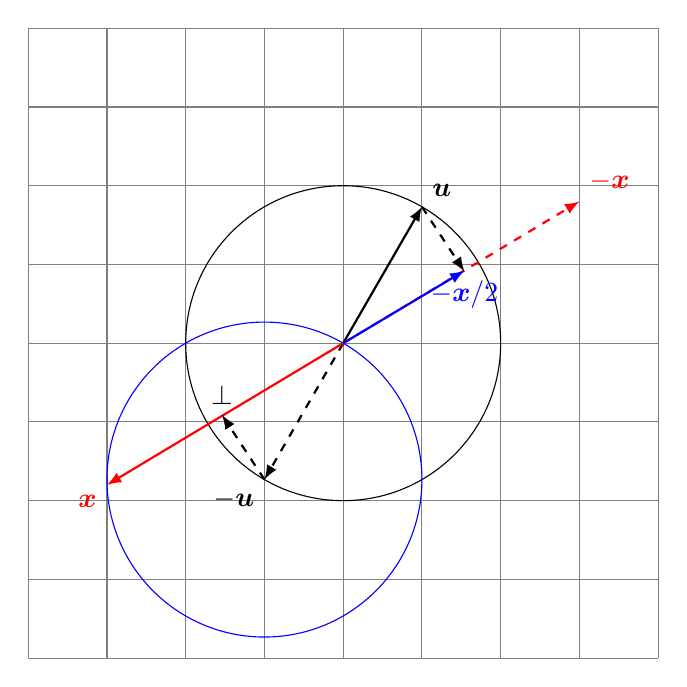
\begin{tikzpicture}
  \tkzInit[xmax=4,ymax=4,xmin=-4,ymin=-4]
  \tkzGrid
  \tkzAxeXY
  % \draw[ thick,-latex] (-6,0) -- (6,0) node [anchor= west]{$x$};
   %\draw[ thick,-latex] (0,-6) -- (0,6) node [anchor= west]{$x$};
   \draw[] (0,0) circle (2);
   \draw[ thick,-latex] (0,0) -- (1,1.732) node [anchor=south west]{$\bm u$};
   \draw[ thick,dashed,-latex] (0,0) -- (-1,-1.732) node [anchor=north east]{$-\bm u$};
   \draw[blue] (-1,-1.732) circle (2);
   \draw[ thick,-latex,red] (0,0) -- (-3,-1.8) node [anchor=north east]{$\bm x$};
   \draw[ thick,dashed,-latex,red] (0,0) -- (3,1.8) node [anchor=south west]{$-\bm x$};
% projection
   \draw[ thick,dashed,-latex] (1,1.732) -- (1.54, 0.91); % the opposite projection
    \draw[ thick,dashed,-latex] (-1,-1.732) -- (-1.54, -0.91) node [anchor=south]{$\perp$};
    \draw[ thick, blue,-latex] (0,0) -- (1.54, 0.92) node [anchor=north]{$-\bm x/2$};    
 % \tkzText[above](0,6.75){2D demo of the basic identity}
  \end{tikzpicture}
\caption{For any point $x$ on the blue circle, the projection point of $u$ on $-x$ should be $-x/2$.}
\label{fig:identity}
\end{center}
\end{figure}


%v' = v - {g\over2} + {r\over2} \omega,\quad v'_* = v - {g\over2} - {r\over2} 

\begin{align}
\begin{split}
Q(f,f)(v) &=  \int_{\mathbb{R}^3} \int_{\mathcal{S}^2} {B}(r,\cos\chi)[f(v_*')f(v')-f(v_*)f(v)] d\omega dv_* \\
& =  \int_{\mathbb{R}^3} \int_{\mathcal{S}^2} {B}(r,\cos\chi) \left[ 
f \left(v_* + {g\over2} - {r\over2} \omega  \right)f \left(v - {g\over2} + {r\over2} \omega \right)  - f(v_*)f(v) \right]  d\omega dv_* \\
& =  \int_{\mathbb{R}^3} \int_{\mathcal{S}^2} {B}(r,\cos\chi) \left[ 
f \left(v_* - {|g|\omega - g\over 2}\right)f \left(v +  {|g|\omega - g\over 2}\right) -f(v_*)f(v)\right]  d\omega dv_* \\
& =  2\int_{\mathbb{R}^3} \int_{\mathbb{R}^3} {1\over r}{B}(r,\cos\chi) \delta\left( 2x\cdot g + |x|^2 \right) \left[ 
f \left(v_* - x/2\right)f \left(v + x/2\right) -f(v_*)f(v)\right]  dx dv_* \\
\end{split}
\end{align}

Change of variable $x \to x/2$ in $x$,
\begin{multline}
Q(f, f)(v) =4 \int_{v_{*} \in \mathbb{R}^{d}} \int_{x \in \mathbb{R}^{d}} B\left(r,\cos\chi\right) \frac{1}{r} \delta\left(4 x \cdot g+4|x|^{2}\right) \\
 \left[f\left(v_{*}-x\right) f(v+x)-f\left(v_{*}\right) f(v)\right] d x d v_{*}
\end{multline}
Let $y = v_* - v - x$, then, 

\begin{multline*}
Q(f, f)(v) =4 \int_{y \in \mathbb{R}^{d}} \int_{x \in \mathbb{R}^{d}} B\left(r,\cos\chi\right) \frac{1}{r} \delta\left(4 x \cdot g+4|x|^{2}\right) \\
 \left[f\left(v+y\right) f(v+x)-f\left(v+x+y\right) f(v)\right] d x d v_{*}
\end{multline*}

\begin{multline*}
Q(f, f)(v) =4 \int_{y \in \mathbb{R}^{d}} \int_{x \in \mathbb{R}^{d}} B\left(r,\cos\chi\right) \frac{1}{r} \delta\left(x \cdot y\right) \\
 \left[f\left(v+y\right) f(v+x)-f\left(v+x+y\right) f(v)\right] d x d y
\end{multline*}

\begin{multline*}
Q(f, f)(v)=4 \int_{y \in \mathbb{R} 3} \int_{x \in \mathbb{R} 3} B\left(|x+y|,-\frac{x \cdot(x+y)}{|x||x+y|}\right) \frac{1}{|x+y|}\delta\left(x \cdot y\right) \\
 \left[f\left(v+y\right) f(v+x)-f\left(v+x+y\right) f(v)\right] d x d y
\end{multline*}
\begin{figure}[tbp]
\begin{center}
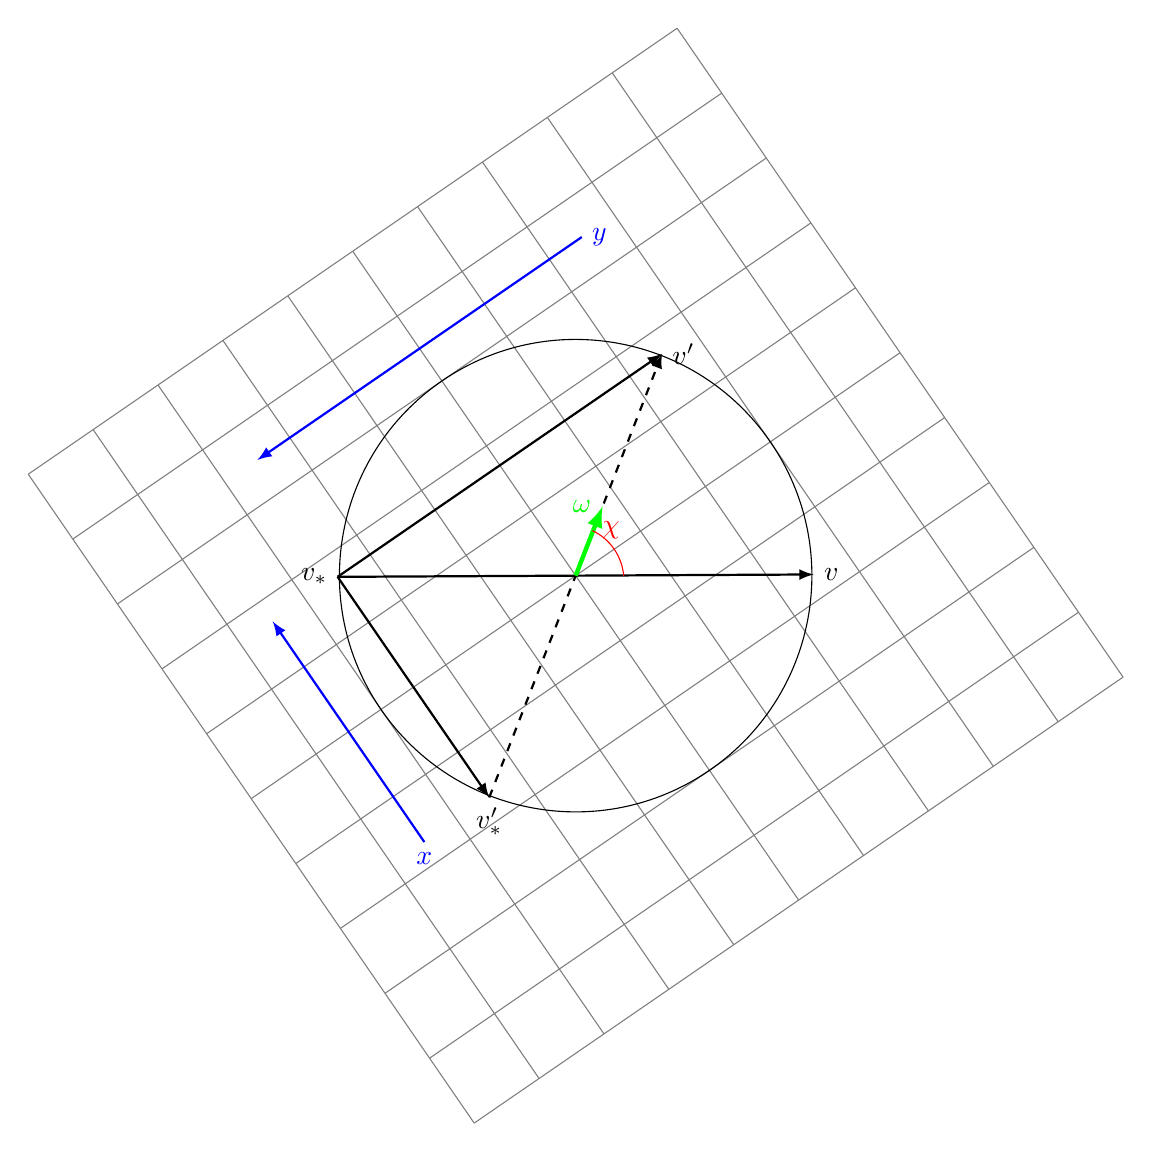
\begin{tikzpicture}[rotate=34.5]
  \tkzInit[xmax=5,ymax=5,xmin=-5,ymin=-5]
  \tkzGrid
  \tkzAxeXY
  % \draw[ thick,-latex] (-6,0) -- (6,0) node [anchor= west]{$x$};
   %\draw[ thick,-latex] (0,-6) -- (0,6) node [anchor= west]{$x$};
   \draw[] (0,0) circle (3);
   
   \draw[thick,-latex] (-2.5,1.7) node[left] {$v_*$}-- (2.5,-1.7) node[right] {$v$};
   \draw[thick,-latex,dashed] (-2.5,-1.7) -- (2.5,1.7);
   \draw[thick,-latex] (-2.5,1.7) -- (-2.5,-1.7) node[below] {$v_*'$};
   \draw[thick,-latex] (-2.5,1.7) -- (2.5,1.7) node[right] {$v'$};
   \draw[thick,latex-, blue] (-3.5,1.7) -- (-3.5,-1.7) node[below] {$x$};
   \draw[thick,latex-, blue] (-2.5,3.5) -- (2.5,3.5) node[right] {$y$};
   \draw[ultra thick,-latex, green] (0,0) -- (0.78,0.531) node [left] {$\omega$} ;
   \draw[red] (0.5,-0.35) arc (-30:30:0.7) node[right] {$\chi$};
   %\tkzDrawArc[0.8 with nodes] ((1,0), 0.5) ((1,-0.7), (1,0.7));
   %\tkzDefPoint (1,0){A}
    %\tkzTangent[from with R=A](O,1cm) \tkzGetPoints{T1}{T2}


   % \draw[ thick, blue,-latex] (0,0) -- (1.54, 0.92) node [anchor=north]{$-\bm x/2$};    
 % \tkzText[above](0,6.75){2D demo of the basic identity}
  \end{tikzpicture}
\caption{Geometry of the collision $\left(v, v_{*}\right) \leftrightarrow\left(v^{\prime}, v_{*}^{\prime}\right)$, $v* = v+x+y$, $v' = v+x$, $v'_* = v+y$. It also indicates $\sin (\chi/2) = |x|/\sqrt{(|x^2|+|y^2|)}$ and $\cos (\chi/2) = |y|/\sqrt{(|x^2|+|y^2|)}$}
\label{fig:collision_geo}
\end{center}
\end{figure}
Define
\begin{equation}\label{tildeB}
\tilde{B}(x, y) \triangleq 4 B\left(|x+y|,-\frac{x \cdot(x+y)}{|x||x+y|}\right)|x+y|^{-1}
\end{equation}
and as $x\cdot y$ = 0, 
\begin{equation*}
\tilde{B}(x, y)=\tilde{B}(|x|,|y|) \triangleq 4 B\left(\sqrt{|x|^{2}+|y|^{2}}, \frac{|x|}{\sqrt{|x|^{2}+|y|^{2}}}\right)\left(|x|^{2}+|y|^{2}\right)^{-\frac{1}{2}}
\end{equation*}

\color{blue}
\begin{align*}\begin{split}
\hat Q[k] &=  \sum_{q=-N/2}^{N/2-1} Q[q]e^{-i{\pi \over L}k\cdot v_q}=   \frac{1}{N^3} \sum_{\substack{l,m= -N/2 \\ l+m = k}}^{N/2-1}\mathcal{G}(l,m)\hat f[l] \hat f[m]  \\
&= \frac{1}{N^3} \sum_{\substack{l,m= -N/2 \\ l+m = k}}^{N/2-1} [G(l,m) - G(m,m)]\hat f[l] \hat f[m]
\end{split}\end{align*}
\color{black}

We can reformulate the integral of $G(l,m)$ of Ref.~ \cite{gambaFastSpectralMethod2017} from the spherical surface integral to 3D Cartesian integral by using the basic identity in Eq.~\eqref{identity};
\begin{align*}
\begin{split}
G(l,m)  &= \int_{\mathbb{R}^3} \int_{\mathcal{S}^2}   B(r,\omega \cdot \hat g)  e^{-i{\pi \over L} \frac{l+m}{2} \cdot g -i {\pi \over L} r \frac{m-l}{2}\cdot \omega}d\omega dg \\
&= \int_{\mathbb{R}^3} \int_{\mathcal{S}^2}   B(r,\omega \cdot \hat g)  e^{-i\frac{\pi}{L}\left[\frac{m-l}{2}\cdot (|g|\omega - g) + m\cdot g\right]} d\omega dg \\
&= 2\int_{\mathbb{R}^3}\int_{\mathbb{R}^3} {1\over r} B(r,\omega \cdot \hat g)  \delta(2x\cdot g + |x|^2) e^{-i\frac{\pi}{L}\left[\frac{m-l}{2}\cdot x + m\cdot g\right]} dx dg \\
&= 2\int_{\mathbb{R}^3}\int_{\mathbb{R}^3}{1\over r} B(r,\omega \cdot \hat g)  \delta(x\cdot y) e^{-i\frac{\pi}{L}\left[\frac{m-l}{2}\cdot x + m\cdot g\right]} dx dg \\
\end{split}
\end{align*}
By change of variable $x \to x/2$ in $x$, and noticing $g = -(x+y)$, it can be further changed the integral of $dxdy$: 

\begin{align*}
\begin{split}
G(l,m) &= 4\int_{\mathbb{R}^3}\int_{\mathbb{R}^3}{1\over r}  B(r,\omega \cdot \hat g)  \delta(x\cdot y) e^{-i\frac{\pi}{L}\left[(m-l)\cdot x + m\cdot g\right]} dx dg \\
&= 4\int_{\mathbb{R}^3}\int_{\mathbb{R}^3}{1\over r}  B(r,\omega \cdot \hat g)  \delta(x\cdot y) e^{i\frac{\pi}{L}(l\cdot x + m\cdot y)} dx dy,
\end{split}
\end{align*}
which is exactly the $\beta(l,m)$ given in Ref.~\cite{mouhotFastAlgorithmsComputing2006}, once using the symbol of $\tilde B(x,y)$ in Eq.~\eqref{tildeB},
\begin{align*}
\begin{split}
G(l,m) &= 4\int_{\mathbb{R}^3}\int_{\mathbb{R}^3} {1\over r}  B(r,\omega \cdot \hat g)  \delta(x\cdot y) e^{-i\frac{\pi}{L}\left[(m-l)\cdot x + m\cdot g\right]} dx dg \\
&= \int_{\mathbb{R}^3}\int_{\mathbb{R}^3} \tilde B(x,y)  \delta(x\cdot y) e^{i\frac{\pi}{L}(l\cdot x + m\cdot y)} dx dy 
\end{split}
\label{eq:Glmxy}
\end{align*}
When $\tilde B(x,y)$ can be decoupled as
\begin{equation*}
\tilde B(x,y) = a(|x|)b(|y|)
\end{equation*} 
then we can have the following decomposition
\begin{equation*}
\mathcal{G}(l,m)  \simeq  \sum_{p=1}\alpha_p(l)\alpha_p'(m).
\end{equation*}
Note, for 2D Maxwell model and 3D HS model, $\tilde B$ is a constant, and such decoupling is straightforward. Thus the convolution computation is of $\hat Q_k$ is possible.

For the 3D case, write Eq.~\eqref{eq:Glmxy} in spherical-coordinate system, $dxdy$ becomes  $\rho^2 \rho^2 d\rho d\rho de de'$. The $\rho^2$ together with $\rho^{-1}$ in $\title{B}$
 leads to $|\rho|$,
\begin{multline}
G(l, m)=\frac{1}{4} \int_{e \in \mathbb{S}^{2}} \int_{e^{\prime} \in \mathbb{S}^{2}} \delta\left(e \cdot e^{\prime}\right) 
\left[\int_{-R}^{R}|\rho| a(\rho) e^{i \frac{\pi}{L} \rho(l \cdot e)} d \rho\right]\left[\int_{-R}^{R}\left|\rho^{\prime}\right| b\left(\rho^{\prime}\right) e^{i \frac{\pi}{L}\rho^{\prime}\left(m \cdot e^{\prime}\right)} d \rho^{\prime}\right] d e ^{\prime}d e
\end{multline}
Define
\begin{equation*}
\phi_{R,a}(s) = \int_{-R}^{R}|\rho| a(\rho) e^{i \rho s} d \rho
\quad
\phi_{R,b}(s) = \int_{-R}^{R}|\rho| b(\rho) e^{i \rho s} d \rho,
\end{equation*}
And they can be further simplied as
 \begin{equation}
\phi_{R,a}(s) = 2\int_0^R\rho a(\rho) \cos(\rho s)d \rho,
\quad
\phi_{R,b}(s) = 2\int_0^R\rho b(\rho) \cos(\rho s)d \rho.
\end{equation}

both of which are odd functions.
Then we have
\begin{multline*}
\begin{split}
G(l, m) &=\frac{1}{4}
 \int_{e \in \mathbb{S}^{2}} \phi_{R,a}\left(\frac{\pi}{L}l\cdot e\right) \int_{e^{\prime} \in \mathbb{S}^{2}} \delta\left(e \cdot e^{\prime}\right)  \left[\int_{-R}^{R}\left|\rho^{\prime}\right| b\left(\rho^{\prime}\right) e^{i \frac{\pi}{L}\rho^{\prime}\left(m \cdot e^{\prime}\right)} d \rho^{\prime}\right] d e ^{\prime}d e \\
 & = \frac{1}{4} \int_{e \in \mathbb{S}^{2}} \phi_{R,a}\left(\frac{\pi}{L}l\cdot e\right) 
 \left[ \int_{e^{\prime} \in \mathbb{S}^{2} \bigcap e^{\perp}}  \phi_{R,b}\left(\frac{\pi}{L}m\cdot e'\right)d e^{\prime}\right]d e
\end{split}
\end{multline*}
The integral of $e'$ in the intersection circle of the unit sphere with the perpendicular plane of  $e$ can be transformed to an integral of over the polar angle in a local polar coordinate system with basis of $(e, u=\Pi_{e^\perp}(m), e\times u)$, where $=\Pi_{e^\perp}(m)$ is the projection vector of $m$ in the perpendicular plane of $e$. The equivalence is
\begin{equation*}
 \int_{e^{\prime} \in \mathbb{S}^{2} \bigcap e^{\perp}}  \phi_{R,b}\left(\frac{\pi}{L}m\cdot e'\right)d e^{\prime}
 = 2 \int_0^{\pi} \phi_{R,b}\left(\frac{\pi}{L} |\Pi_{e^{\perp}}(m)| \cos \theta' \right) d \theta' 
 \end{equation*}
 in which the odd function property of $\phi_{R,b}$ is used. 
\begin{figure}[tbp]
\begin{center}
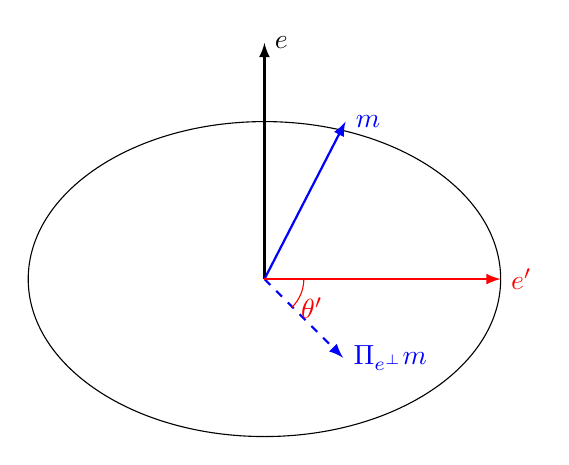
\begin{tikzpicture}[rotate=0]
   \draw[] (0,0) ellipse (3 and 2);
   \draw[thick,-latex] (0,0) -- (0,3) node[right]{$e$};
   \draw[thick,-latex, blue] (0,0) -- (1.03,2) node[right]{$m$};
   \draw[thick,dashed,-latex, blue] (0,0) -- (1.0,-1) node[right]{$\Pi_{e^{\perp}}m$};
   \draw[thick,-latex, red] (0,0) -- (3,0) node[right]{$e'$};
   \draw[red] (0.5,0) arc (0:-47:0.5) node[right] {$\theta'$};
\end{tikzpicture}
\caption{Geometry}
\label{fig:local_polar_coordinate}
\end{center}
\end{figure}
Define
\begin{equation*}
\psi_{R,b}\left(\Pi_{e^{\perp}}\left(\frac{\pi}{L}m \right) \right ) \triangleq \int_0^{\pi}  \phi_{R,b}\left( \left\vert\Pi_{e^{\perp}}\left(\frac{\pi}{L}m \right) \right \vert \cos \theta' \right) d \theta' 
\end{equation*}
Thus we have
\begin{multline*}
\begin{split}
G(l, m)
 & = \int_{e \in \mathbb{S}^{2}_+} \phi_{R,a}\left(\frac{\pi}{L}l\cdot e\right) 
 \psi_{R,b}\left(\Pi_{e^{\perp}}(\frac{\pi}{L}m)\right)  de
\end{split}
\end{multline*}
The surface integral is approximated numerically by taking a spherical parameterizations of $(\theta', \varphi)$ of $e \in \mathbb{S}^{2}_+$ and uniform grids of size $M_1$ and $M_2$,
\begin{equation*}
G(l, m)
  = \frac{\pi^2}{M_1M_2}\sum_{p,q=0}^{M1,M2} \phi_{R,a}\left(\frac{\pi}{L}l\cdot e_{(\theta'_p,\varphi_q)}\right) 
 \psi_{R,b}\left(\Pi_{e^{\perp}_{(\theta'_p,\varphi_q)}}\left(\frac{\pi}{L}m \right) \right)
 \end{equation*}
 and
 \begin{equation*}
 \left(\theta'_{p}, \varphi_{q}\right)=\left(\frac{p \pi}{M_{1}}, \frac{q \pi}{M_{2}}\right)
 \end{equation*}
 Define
 \begin{equation*}
 \alpha_{p, q}(l)=\phi_{R, a}\left(\frac{\pi}{L}l \cdot e_{\left(\theta'_{p}, \varphi_{q}\right)}\right), \quad \alpha_{p, q}^{\prime}(m)=\psi_{R, b}\left(\Pi_{e_{(\theta'_p, \varphi_{q})} }\left(\frac{\pi}{L}m \right)\right)
 \end{equation*}
We have
\begin{equation*}
G(l, m)
  = \frac{\pi^2}{M_1M_2}\sum_{p,q=1}^{M1,M2}\alpha_{p,q}(l) \alpha'_{p,q}(m).
 \end{equation*}
When $|a(\rho)|  = |b(\rho)|= 1$,
\begin{equation*}
\phi_{R,1}(s) = R^2[2\Sinc(Rs) - \Sinc^2(Rs/2)]
\end{equation*}
Thus, in the implementation, $\phi_{R,a}$ can be computed `on-the-fly', while $\phi_{R,a}\left(\frac{\pi}{L}l\cdot e\right)$ can be pre-computed for all discrete $m$ and $e$ and stored for reused. 
Note, we can further simplify $\psi_{R,b}$ into a single integration in $d\rho$ as
\begin{multline*}
\begin{split}
\psi_{R,b}\left(\Pi_{e^{\perp}}\left(\frac{\pi}{L}m \right) \right ) &\triangleq \int_0^{\pi}  \phi_{R,b}\left( \left\vert\Pi_{e^{\perp}}\left(\frac{\pi}{L}m \right) \right \vert \cos \theta' \right) d \theta'  \\ 
&  = 2\pi \int_0^R \rho  b(\rho ) J_0\left(\rho\left \vert \Pi_{e^{\perp}}\left(\frac{\pi}{L}m \right) \right \vert \right) d\rho
\end{split}
\end{multline*}
in which  we have used the zero-order Bessel function. The integral representation of Bessel function is 
\begin{equation*}
J_{\alpha}(x)=\frac{1}{ \pi} \int_{0}^{\pi} \cos (\alpha \tau-x \sin \tau) d \tau.
\end{equation*}
In particular, the zero-order Bessel function is
\begin{equation}
J_{0}(x)=\frac{1}{\pi} \int_{0}^{\pi} \cos(x \sin \tau) d \tau = \frac{1}{\pi} \int_{0}^{\pi} \cos(x \cos \tau) d \tau
\end{equation}

\section{Wu's JCP2013 Paper}

\subsubsection{Special case of Maxwell molecules, $\alpha,\gamma=0$}

The generalized collision kernel in Wu's paper is
\begin{equation}
B(r,\cos \chi) = C^{''}_{\gamma,\alpha}\sin^{\gamma+\alpha-1}\left ( {\chi \over 2}\right)\cos^{-\alpha}\left ( {\chi \over 2}\right)r^{\gamma}
\end{equation}
in which we have used the reversed notation as in Wu's paper, i.e., $\gamma$ changed to $\alpha$, and $\alpha$ changed to $\gamma$. For the special case of $\alpha,\gamma=0$, we have the constant collision kernel for Maxwell molecules:
\begin{equation}
B_\text{Maxwell} =   C^{''}_{\gamma,\alpha} \sin^{-1}\left ( {\chi \over 2}\right)
\end{equation}

Use Mouhot's notations,
\begin{equation*}
a(\rho) = |\rho|^{-1},\quad b(\rho) = 1
\end{equation*}

\begin{align*}
\begin{split}
\phi_{R, a}(s) &=\phi_{R, 0}(s)  =  2 \int_{0}^{R} \cos (\rho s) d \rho = 2\Sinc(Rs)\\
\phi_{R, b}(s) &=\phi_{R, 1}(s) =  2 \int_{0}^{R} \rho \cos (\rho s) d \rho = R^2[2\Sinc(Rs) - \Sinc^2(Rs/2)]
\end{split}
\end{align*}

\begin{multline*}
\begin{split}
\psi_{R,b}\left(\Pi_{e^{\perp}}\left(\frac{\pi}{L}m \right) \right ) &=\psi_{R,1}\left(\Pi_{e^{\perp}}\left(\frac{\pi}{L}m \right) \right )   \\
& = \int_0^{\pi}  \phi_{R,1}\left( \left\vert\Pi_{e^{\perp}}\left(\frac{\pi}{L}m \right) \right \vert \cos \theta' \right) d \theta'  \\ 
&  = 2\pi \int_0^R \rho J_0\left(\rho\left \vert \Pi_{e^{\perp}}\left(\frac{\pi}{L}m \right) \right \vert \right) d\rho
\end{split}
\end{multline*}

\begin{equation}
\int_0^R \rho J_0(s\rho) = {1\over s^2}\int_0^{sR}t J_0(t) dt
\end{equation}

In Wolfram documentation
\begin{equation}
\int z J_0(z) dz = {z^2\over 2} F_2\left( 1; 1,2;-z^2/4\right)
\end{equation}
where $F_2(\{a_1,\dots,a_p\}, \{a_1,\dots,a_p\}, z)$ is the \verb|HypergeometricPFQ| function

Some integral
\begin{equation*}
{1\over 2}\int_0^\pi \sin^{-1}(\theta/2)\sin^3(\theta)d\theta = \frac{16}{15}
\end{equation*}



\bibliographystyle{amsplain}

%\bibliographystyle{te}
\bibliography{FSM}
\end{document} 
